\chapter{Curve Theory}

\section{Regular Curve}

\definition{Regular Curve}\\
A curve $\alpha:[c,d]\to\mathbb{R}^3$ is said to be \textit{regular} if the derivative does not vanish in the sense of norm, i.e.: on $[c,d]$
\[
|\alpha'| \neq 0
\]
($\alpha$ is taken to be differentiable).

\begin{proposition}{Riemann Sum and Arc-length of Regular Curve}\\
Let $\alpha:[c,d]\to\mathbb{R}^3$ be a regular curve with partition $\mathcal{P}=\{c=t_0<t_1<\cdots<t_n=d\}$ and let 
\[
l(\alpha,\mathcal{P}):=\sum_{i=0}^{n-1}|\alpha(t_i)-\alpha(t_{i+1})|
\]
Then the arc-length of $\alpha$ is equal to
\[
\int_c^d\left|\frac{d\alpha}{dt}\right| dt = \sup\left\{l(\alpha,\mathcal{P})\mid\mathcal{P}\text{ any partition of }[c,d]\right\}
\]
\end{proposition}

\begin{proposition}{Well-defined-ness of Regular Curve}\\
Let $\alpha:[a,b]\to\mathbb{R}^3$ be a regular curve and let $g:[c,d]\to[a,b]$ be a reparametrization with $\beta=\alpha\circ g$. Then:
\[
\int_a^b\left|\frac{d\alpha}{dt}\right| dt = \int_c^d\left|\frac{d\beta}{ds}\right| ds
\]
\end{proposition}

\begin{proof} 
It immediately follows from the Chain Rule.
\end{proof}

\section{Local Theory of Curves}

\subsection{Intuition and Basic Concepts}


\noindent\textbf{Intuition:} There are many ways to parametrize the same curve, but we want to pick one such that the ``tangent'' is moving at \textit{unit} speed, i.e.: $\forall a\le s\le b$, $|\frac{d\beta}{ds}|=1$, or equivalently, $\forall a\le s\le b$,
\[
\int_a^b\left|\frac{d\beta}{ds}\right| ds = b - a
\]

\definition{Plane Curve}\\
The \textit{trace} of a curve $\alpha$ is defined to be $\mathrm{im}(\alpha)$ ($\subseteq \mathbb{R}^3$). If $\mathrm{im}(\alpha)$ lies on a plane $P\subseteq\mathbb{R}^3$, then $\alpha$ is called a \textit{plane curve}.

\noindent\textbf{Remark:} By default, we express our vector in $\mathbb{R}^3$ by the usual basis
\[
\mathcal{A} := \left\{\begin{pmatrix}0\\0\\1\end{pmatrix}, \begin{pmatrix}1\\0\\0\end{pmatrix}, \begin{pmatrix}0\\1\\0\end{pmatrix}\right\}
\]
i.e.: $\alpha=(x(t),y(t),z(t))_{\mathcal{A}} = \begin{pmatrix}x(t)\\y(t)\\z(t)\end{pmatrix}_{\mathcal{B}}$. However, our results also hold by using coordinate vectors of another orthonormal basis $\mathcal{B}=\{u_1, u_2, u_3\}$.

\noindent If $\alpha$ is a plane curve, i.e.: $\alpha(t)\in P$ with $P=\{z_0+pu_1+gu_2\mid p,g\in\mathbb{R}\}$, then
\[
\alpha(t) = (z_0)_{\mathcal{B}} + (a(t), b(t),0)_{\mathcal{B}} \in\mathbb{R}^3
\]

\noindent To simplify further, one can just study the curve $\beta:I\to\mathbb{R}^2$ given by $\beta(t):=(a(t),b(t))$, and then all our results on plane curves can be obtained from $\alpha: I\xrightarrow{\beta}\mathbb{R}^2\xrightarrow{\gamma}\mathbb{R}^3$ where $\gamma (a,b)=(a,b,0)_{\mathcal{B}}=au_1+bu_2$.

\definition{Tangent Vector}\\
Let the curve $\alpha:I\to\mathbb{R}^3$ be regular. The \textit{velocity vector} of $\alpha$ at $t\in I$ is given by $\alpha'(t)$ and the \textit{speed} of $\alpha$ at $t\in I$ is given by $|\alpha'(t)|$. Then we define the \textit{tangent vector} $T(t)$ of $\alpha$ by
\[
T(t) := \frac{\alpha'(t)}{|\alpha'(t)|}
\]

\noindent Furthermore, the tangent line at $t=t_0$ is: $l(t_0) := \alpha(t_0)+\lambda T(t_0)$.

\noindent\textbf{Remark:} The cusp is not a regular curve since $|\alpha'(0)|=0$, but we allow self-intersection, i.e.: $\exists t_1\neq t_2$ s.t.: $\alpha(t_1)=\alpha(t_2)$. Moreover, they are also allowed to have different tangent vectors $T(t_1)\neq T(t_2)$.

\subsection{Reparametrization}

\definition{Reparametrization}\\
The \textit{reparametrization} of a curve $\alpha:[a,b]\to\mathbb{R}^3$ is a bijective function $g:[c,d]\to[a,b]$ such that $g$ is $\mathcal{C}^\infty$ and $g^{-1}$ is $\mathcal{C}^1$ (differentiable with continuous derivative).

\begin{proposition}{Invariance of Regularity under Reparametrization}\\
If $\alpha$ is a regular curve and $g$ is a reparametrization, then $\beta := \alpha\circ g$ is regular.
\end{proposition}

\begin{proof}
Note that $g\circ g^{-1} = \mathrm{id}$. Hence, $g'(g^{-1}(t))\cdot(g^{-1})'(t) = 1, \forall t$. Therefore, by the bijectivity of $g$, $g'(s)\neq 0$, $\forall s$. Thus,
\[
|\beta'(s)| = |\alpha'(g(s))|\cdot|g'(s)| \neq 0.
\]
\end{proof}

\begin{proposition}{``Invariance'' of Tangent Vector under Reparametrization}\\
Let $\alpha$ be a regular curve and let $g$ be a reparametrization with $\beta = \alpha\circ g$. If $T$ is the tangent vector of $\alpha$ at $t = g(s_0)$ and if $S$ is the tangent vector of $\beta$ at $s = s_0$, then
\[
S = \mathrm{sgn}\left(\frac{dg}{ds}\bigg|_{s_0}\right)\cdot T
\]
\end{proposition}

\begin{proof}
Note that $g'(s_0)/|g'(s_0)| = \mathrm{sgn}(g'(s_0))$. Hence, by chain rule, we're done.
\end{proof}

\subsection{Arc-length}

\begin{proposition}{Basic Formula for computing Arc-length}\\
\[
\int_\alpha ds = \int_c^d\left|\frac{d\alpha}{dt}\right| dt = \int_c^d\sqrt{(x')^2+(y')^2+(z')^2}\ dt
\]
\end{proposition}

\noindent\textbf{Remark:} $\sqrt{(x')^2+(y')^2+(z')^2} = ds$

\begin{proposition}{Invariance of Arc-length under Reparametrization}\\
Let $\alpha$ be a regular curve and let $g$ be a reparametrization with $\beta = \alpha\circ g$. Then
\[
\int_\alpha dt = \int_\beta ds
\]
\end{proposition}

\lemma{Preparation for defining Arc-length Parametrization}\\
Let $t_0\in[a,b]$. Consider $h:[a,b]\to\mathbb{R}$ given by
\[
h(t) := \int_{t_0}^t \left|\frac{d\alpha}{ds}\right| ds
\]
Then:
\begin{itemize}
\item $h:[a,b]\to[h(a),h(b)]$ is $\mathcal{C}^\infty$
\item $h^{-1}$ exists and is also $\mathcal{C}^\infty$
\end{itemize}

\begin{proof}
The second property is immediately from IVT.
\end{proof}

\definition{Arc-length Parametrization}\\
Let $\alpha:[a,b]\to\mathbb{R}^3$ be regular and $t_0\in I$ with $g=h^{-1}$ a reparametrization, where $h$ is given in the Preparation for defining Arc-length Parametrization lemma. Then $\beta=\alpha\circ g:[h(a),h(b)]\to\mathbb{R}^3$ is \textit{parametrization by arc-length} (\textit{p.a.l.}).

\begin{proposition}{Advantage of P.A.L.}\\
Let $\beta$ be a p.a.l. Then $|d\beta/ds| = 1$.
\end{proposition}

\begin{proof}
$|d\beta/ds| = |\beta'(g(s))|\cdot|g'(s)| = |h'|\cdot\frac{1}{|h'|} = 1$.
\end{proof}

\begin{corollary}{of Advantage of P.A.L. Proposition}\\
If $\beta$ is a p.a.l., then $\beta' = T$.
\end{corollary}

\subsection{Frenet Frame and Curvature of plane curve}

\noindent In this section, we assume $\alpha:I\to\mathbb{R}^2$ where $\alpha$ is a p.a.l.

\definition{Normal Vector}\\
The \textit{normal vector} $N(s)$ of $\alpha$ at $t=s$ is the vector
\[
N(s) := J(T(s))
\]
where $J$ is the $90^\circ$ anticlockwise rotation $\begin{pmatrix}0 & -1\\1 & 0\end{pmatrix}$, i.e.: $J:\begin{pmatrix}a\\b\end{pmatrix}\mapsto\begin{pmatrix}-b\\a\end{pmatrix}$. 

\begin{definition}{Frenet Frame}\\
The set $\{T(s),N(s)\}$ forms an ordered, oriented basis of $\mathbb{R}^2$ which is orthonormal. It's called the \textit{Frenet frame} of $\alpha$.
\end{definition}

\definition{Curvature}\\
Since $\langle T(s), T(s)\rangle = 1$, then $2\langle T'(s), T(s)\rangle = \frac{d}{ds}\langle T(s), T(s)\rangle = 0$, so there must be some scalar $K(s)$, s.t.: $T'(s) = K(s)N(s)$. The \textit{curvature} of $\alpha$ at $s$ is the value $K(s)$.

\begin{proposition}
$N'(s) = -K(s)T(s)$.
\end{proposition}

\begin{proof}
\textbf{Method 1}: Since $\langle N(s), N(s)\rangle = 1$, then $2\langle N'(s), N(s)\rangle = 0$, so there must be some scalar $c(s)$, s.t.: $N'(s) = c(s)T(s)$. Since $\langle T(s), N(s)\rangle = 0$, then
\[
0 = \frac{d}{ds}\langle T(s), N(s)\rangle = \langle T'(s), N(s)\rangle + \langle T(s), N'(s)\rangle
\]
Hence,
\[
0 = \langle K(s)N(s), N(s)\rangle + \langle T(s), c(s)T(s)\rangle = K(s) + c(s).
\]

\noindent\textbf{Method 2}: Note that
\[
J^2 = \begin{pmatrix}0 & -1\\1 & 0\end{pmatrix}^2 = \begin{pmatrix}-1 & 0\\0 & -1\end{pmatrix} = -I.
\]
Hence,
\[
N'(s) = \frac{d}{ds}J(T(s)) = J(T'(s)) = J(K(s)N(s)) = K(s)J(N(s)) = K(s)J(J(T(s))) = K(s)\cdot(-T(s)).
\]
\end{proof}

\noindent\textbf{Remark:} $K(s)$ records ``the change of $T(s)$'':

\noindent\begin{itemize}
\item $K(s)\equiv 0 \iff T'(s)\equiv 0 \iff T(s) = \underline{v}$ for some constant vector $\underline{v}$.
\item $K(s) > 0 \Rightarrow T(s)$ is turning towards $N(s)$, say, $T'$ along the direction of $N$.
\item $K(s) < 0 \Rightarrow T(s)$ is turning away $N(s)$, say, $T'$ against the direction of $N$.
\end{itemize}

\noindent\textbf{Example}: Let $\alpha(s) := \underline{u} + r\left(\cos\frac{s}{r}, \sin\frac{s}{r}\right)$ be a circle centered at $\underline{u}$ of radius $r$. Then
\[
T_\alpha(s) := \alpha'(s) = \left(-\sin\frac{s}{r}, \cos\frac{s}{r}\right) \Rightarrow N_\alpha(s) := J(T_\alpha(s)) = \left(-\cos\frac{s}{r}, -\sin\frac{s}{r}\right)
\]
and $T_\alpha'(s) = \frac{1}{r}\left(-\cos\frac{s}{r}, -\sin\frac{s}{r}\right)$. Hence, by the def of curvature, $K_\alpha(s) = \frac{1}{r}$.

\noindent By contrast, consider $\beta(s) := \underline{u} + r\left(\cos(-\frac{s}{r}), \sin(-\frac{s}{r})\right)$, which is the opposite orientation of the above circle $\alpha$. Then after a simple computation, we have $K_\beta(s) = -\frac{1}{r}$.

\begin{proposition}{Curvature Formula for Regular Plane Curve}\\
Let $\alpha: I\to\mathbb{R}^2$ be a regular curve with p.a.l. $\beta = \alpha\circ g$. Then the curvature of $\alpha$ is:
\[
K_\alpha(s) := \frac{\det(\alpha'(t), \alpha''(t))}{|\alpha'(t)|^3}
\]
where $t = g(s)$.
\end{proposition}

\begin{proof}
By the def of p.a.l., $\frac{ds}{dt} = \frac{d}{dt}(g^{-1}(t)) = |\alpha'(t)|$. Hence,
\[
\frac{dt}{ds} = \frac{1}{|\alpha'(t)|}
\]
Then by the Chain Rule,
\[
\beta'(s) = \alpha'(t)\frac{dt}{ds} = \frac{\alpha'(t)}{|\alpha'(t)|}
\]
and then
\[
\beta''(s) = \frac{d}{ds}\frac{\alpha'(t)}{|\alpha'(t)|} = \frac{dt}{ds}\frac{d}{dt}\frac{\alpha'(t)}{|\alpha'(t)|} = \frac{1}{|\alpha'(t)|}\cdot\frac{\alpha''(t)|\alpha'(t)| - \alpha'(t)\cdot\frac{d}{dt}|\alpha'(t)|}{|\alpha'(t)|^2}
\]
Since $\{T_\beta, N_\beta\}$ is orthonormal, then $\det(T_\beta(s), N_\beta(s)) = 1$, $\forall s$. Hence,
\[
K_\beta(s) = K_\beta(s)\det(T_\beta(s), N_\beta(s)) = \det(T_\beta(s), K_\beta(s)N_\beta(s)) := \det(T_\beta(s), T_\beta'(s))
\]
\[
:= \det(\beta'(s), \beta''(s)) = \det\left(\frac{\alpha'(t)}{|\alpha'(t)|}, \frac{\alpha''(t)|\alpha'(t)| - \alpha'(t)\cdot\frac{d}{dt}|\alpha'(t)|}{|\alpha'(t)|^3}\right)
\]
\[
= \det\left(\frac{\alpha'(t)}{|\alpha'(t)|}, \frac{\alpha''(t)}{|\alpha'(t)|^2}\right) - \det\left(\frac{\alpha'(t)}{|\alpha'(t)|}, \frac{\alpha'(t)\cdot\frac{d}{dt}|\alpha'(t)|}{|\alpha'(t)|^3}\right)
\]
\[
= \det\left(\frac{\alpha'(t)}{|\alpha'(t)|}, \frac{\alpha''(t)}{|\alpha'(t)|^2}\right) - \frac{\frac{d}{dt}|\alpha'(t)|}{|\alpha'(t)|^4}\cdot\det(\alpha'(t), \alpha'(t))
\]
\[
= \frac{1}{|\alpha'(t)|^3}\det(\alpha'(t), \alpha''(t)) - 0
\]
\end{proof}

\subsection{Fundamental Theorem for Plane Curve}

\definition{Orthogonal Group}\\
We define the \textit{orthogonal group} and \textit{special orthogonal group} by
\[
O(n) := \{A\in M_{n\times n}(\mathbb{R}) \mid A^TA = I\}
\]
respectively
\[
SO(n) := \{A\in M_{n\times n}(\mathbb{R}) \mid A^TA = I, \det(A) = 1\}
\]

\noindent\textbf{Example}: $n = 2$.
\[
SO(2) = \left\{\begin{pmatrix}\cos\theta & -\sin\theta\\ \sin\theta & \cos\theta\end{pmatrix}\right\}
\]
consists of {rotation matrices}, and
\[
O(2) = \left\{\begin{pmatrix}\cos\theta & -\sin\theta\\ \sin\theta & \cos\theta\end{pmatrix}, \begin{pmatrix}\cos\theta & \sin\theta\\ \sin\theta & -\cos\theta\end{pmatrix}\right\} = \text{``rotation''} + \text{``reflection''}.
\]

\begin{proposition}{Orthonormal Basis preserving Orthogonality}\\
If $\{\underline{u}_1, \cdots, \underline{u}_n\}$ is an orthonormal basis of $\mathbb{R}^n$ under usual dot product, and if $A\in O(n)$, then so is $\{A\underline{u}_1, \cdots, A\underline{u}_n\}$.
\end{proposition}

\begin{proof}
$\forall i, j$,
\[
\langle A\underline{u}_i, A\underline{u}_j\rangle = (A\underline{u}_i)^T A\underline{u}_j = \underline{u}_i^T A^T A\underline{u}_j = \underline{u}_i^T\underline{u}_j = \langle\underline{u}_i, \underline{u}_j\rangle = \begin{cases}1, & \text{if } i = j\\ 0, & \text{if } i\neq j\end{cases}
\]
\end{proof}

\definition{Rigid Motion}\\
We say a map $\mathbb{R}^n\to\mathbb{R}^n$ is a \textit{rigid motion} if it is of the form:
\[
\underline{x}\mapsto A\underline{x} + \underline{b}
\]
where $A\in O(n)$ and $\underline{b}\in\mathbb{R}^n$. Furthermore, if $A\in SO(n)$, then we call the rigid motion \textit{orientation preserving}.

\theorem{Fundamental Theorem for Plane Curve}
\begin{enumerate}
\item (Existence). For any $\mathcal{C}^\infty$ function $f: I\to\mathbb{R}$, $\exists$ p.a.l. plane curve $\alpha: I\to\mathbb{R}^2$, s.t.:
\[
K_\alpha(s) = f(s) \quad\forall s\in I, \text{ with } \alpha(0) = x_0
\]
\item (Uniqueness). Suppose that there are two curves $\alpha, \alpha^*$ p.a.l., s.t.: $K_\alpha = K_{\alpha^*}$, $\forall s\in I$, then they only differ by a rigid motion, i.e.: $\alpha^* = \Phi\circ\alpha$ for some $\Phi: \mathbb{R}^2\to\mathbb{R}^2$ rigid motion.
\end{enumerate}

\begin{proof} \begin{enumerate}
    \item Consider a system of ODE
\[
\begin{cases}
t'(s) = f(s)n(s)\\
n'(s) = -f(s)t(s)
\end{cases}
\iff
\begin{pmatrix}t\\n\end{pmatrix}' = \begin{pmatrix}0 & f\\-f & 0\end{pmatrix}\begin{pmatrix}t\\n\end{pmatrix}
\]
with $t(0) = p\neq 0$ unit length and $n(0) = q = \begin{pmatrix}0 & -1\\1 & 0\end{pmatrix}p$. Then by the existence and uniqueness of ODE solutions give a unique solution for $t$ and $n$.

\noindent Since
\[
\frac{d}{ds}\langle t, n\rangle = \langle t', n\rangle + \langle t, n'\rangle = \langle fn, n\rangle + \langle t, -ft\rangle = f(\langle n, n\rangle - \langle t, t\rangle)
\]
and
\[
\frac{d}{ds}\langle t, t\rangle = \langle t', t\rangle + \langle t, t'\rangle = 2f\langle t, n\rangle \quad\text{and}\quad \frac{d}{ds}\langle n, n\rangle = -2f\langle t, n\rangle
\]
then if we denote $a(s) := \langle t(s), t(s)\rangle$, $b(s) := \langle t(s), n(s)\rangle$, and $c(s) := \langle n(s), n(s)\rangle$, then we obtain another ODE system
\[
\begin{cases}
a' = 2fb\\
b' = f(c - a)\\
c' = -2fb
\end{cases}
\]
with initial value $(a(0), b(0), c(0)) = (1, 0, 1)$. Note that $(a, b, c)\equiv(1, 0, 1)$ satisfies this system, so by the existence and uniqueness of ODE solutions, $\langle t(s), t(s)\rangle\equiv 1$, $\langle t(s), n(s)\rangle\equiv 0$, and $\langle n(s), n(s)\rangle\equiv 1$.

\noindent Then we define $\alpha(s) := x_0 + \int_0^s t(\sigma)\,d\sigma$. We can check:
\begin{itemize}
\item $\alpha(0) = x_0$
\item $\alpha'(s) = t(s)$.
\item Since $|\alpha'(s)| = |t(s)| = \langle t, t\rangle\equiv 1$, then $\alpha$ is a p.a.l.
\item $T_\alpha'(s) := \alpha''(s) = t'(s) = f(s)n(s)$
\end{itemize}

\noindent Hence, by def, it remains to show that $n(s) = N_\alpha(s)$: Since $\langle t, n\rangle\equiv 0$, then $n(s) = J(t(s))$ or $n(s) = -J(t(s))$, where $J = \begin{pmatrix}0 & -1\\1 & 0\end{pmatrix}$. Note that when $s = 0$, $n(0) = \begin{pmatrix}0 & -1\\1 & 0\end{pmatrix}t(0) = q$, i.e.: the first case holds at $s = 0$. Moreover, note that the function $\|n(s) - \begin{pmatrix}0 & -1\\1 & 0\end{pmatrix}t(s)\|$ is continuous, so we must have
\[
n(s) = \begin{pmatrix}0 & -1\\1 & 0\end{pmatrix}t(s)
\]
Since $T_\alpha(s) := \alpha'(s) = t(s)$, then by def, $n(s) = N_\alpha(s)$.

    \item Denote $K(s) := K_\alpha(s) = K_{\alpha^*}(s)$, $\forall s\in I$. Let $A\in SO(2)$ be such that
\[
\begin{pmatrix}T_{\alpha^*}(0)\\ N_{\alpha^*}(0)\end{pmatrix} = A\begin{pmatrix}T_\alpha(0)\\ N_\alpha(0)\end{pmatrix}
\]
and let $b := \alpha^*(0) - A\alpha(0)$. Consider $\Phi(x) := Ax + b$ and $\tilde{\alpha} := \Phi\circ\alpha$. Then
\[
\|\tilde{\alpha}'(s)\| = \left\|\frac{d}{ds}(A\alpha(s) + b)\right\| = \|A\alpha'(s)\| = 1
\]
since $A\in SO(2)$ and $\alpha$ is p.a.l. Hence, $\tilde{\alpha}$ is a p.a.l.

\noindent $\tilde{\alpha}' = A\alpha' \Rightarrow T_{\tilde{\alpha}} = AT_\alpha \Rightarrow K_{\tilde{\alpha}}N_{\tilde{\alpha}} = T_{\tilde{\alpha}}' = AT_\alpha' = AK N_\alpha$
\[
\Rightarrow K_{\tilde{\alpha}}N_{\tilde{\alpha}} = KA\begin{pmatrix}0 & -1\\1 & 0\end{pmatrix}T_\alpha = K\begin{pmatrix}0 & -1\\1 & 0\end{pmatrix}AT_\alpha = K\begin{pmatrix}0 & -1\\1 & 0\end{pmatrix}T_{\tilde{\alpha}} = KN_{\tilde{\alpha}}
\]
\[
\Rightarrow K_{\tilde{\alpha}} = K \quad\quad (*)
\]
Now consider $f(s) := \langle T_{\tilde{\alpha}}, T_{\alpha^*}\rangle + \langle N_{\tilde{\alpha}}, N_{\alpha^*}\rangle$. Then
\[
f'(s) = \frac{d}{ds}\left(\langle T_{\tilde{\alpha}}, T_{\alpha^*}\rangle + \langle N_{\tilde{\alpha}}, N_{\alpha^*}\rangle\right) = \langle T_{\tilde{\alpha}}', T_{\alpha^*}\rangle + \langle T_{\tilde{\alpha}}, T_{\alpha^*}'\rangle + \langle N_{\tilde{\alpha}}', N_{\alpha^*}\rangle + \langle N_{\tilde{\alpha}}, N_{\alpha^*}'\rangle
\]
\[
= \langle K_{\tilde{\alpha}}N_{\tilde{\alpha}}, T_{\alpha^*}\rangle + \langle T_{\tilde{\alpha}}, KN_{\alpha^*}\rangle + \langle -K_{\tilde{\alpha}}T_{\tilde{\alpha}}, N_{\alpha^*}\rangle + \langle N_{\tilde{\alpha}}, -KT_{\alpha^*}\rangle
\]
\[
\stackrel{(*)}{=} K\left(\langle N_{\tilde{\alpha}}, T_{\alpha^*}\rangle + \langle T_{\tilde{\alpha}}, N_{\alpha^*}\rangle - \langle T_{\tilde{\alpha}}, N_{\alpha^*}\rangle - \langle N_{\tilde{\alpha}}, T_{\alpha^*}\rangle\right) = 0.
\]
Hence, $f(s) = $ constant. By the def of $A$, $T_{\tilde{\alpha}}(0) = AT_\alpha(0) = T_{\alpha^*}(0)$ and $N_{\tilde{\alpha}}(0) = AN_\alpha(0) = N_{\alpha^*}(0)$. Thus
\[
f(s)\equiv f(0) = \langle T_{\alpha^*}(0), T_{\alpha^*}(0)\rangle + \langle N_{\alpha^*}(0), N_{\alpha^*}(0)\rangle = 1+1 = 2.
\]
Since $T_{\tilde{\alpha}}$, $T_{\alpha^*}$, $N_{\tilde{\alpha}}$ and $N_{\alpha^*}$ are unit vectors, then $T_{\tilde{\alpha}}(s) = T_{\alpha^*}(s)$ and $N_{\tilde{\alpha}}(s) = N_{\alpha^*}(s)$, $\forall s\in I$. Integrate $T_{\tilde{\alpha}}(s) = T_{\alpha^*}(s)$ and substitute the initial condition $\tilde{\alpha}(0) = A\alpha(0) + b = \alpha^*(0)$. Then we get $\tilde{\alpha}(s) = \alpha^*(s)$, $\forall s\in I$, that is, $\alpha^* = \Phi\circ\alpha$.
\end{enumerate}
\end{proof}


\subsection{Space Curve}

\definition{Frenet-Serret Frame}\\
Let $\alpha: I\to\mathbb{R}^3$ be a regular p.a.l. Define the \textit{tangent vector} of $\alpha$ by $T(s) := \alpha'(s)$. Furthermore, if $T'(s)\neq 0$, then we define
\begin{itemize}
\item \textit{normal vector}: $N(s) := T'(s)\big/\|T'(s)\|$.
\item \textit{binormal vector}: $B(s) := T(s)\times N(s)$.
\end{itemize}
The \textit{Frenet-Serret frame} of $\alpha$ is the orthonormal basis $\{T, N, B\}$.

\noindent\textbf{Rmk:} Unlike the case of plane curve, the normal vector $N$ is simply along the same direction of $T'$, so the curvature is always positive.

\definition{Curvature}\\
The \textit{curvature} of a regular p.a.l. is defined by $K(s) := \|T'(s)\|$.

\definition{Torsion}\\
Since $\langle B, B\rangle = 1$, then $0 = 2\langle B', B\rangle$, so $B'\perp B$. On the other hand, since
\[
B' = T'\times N + T\times N' = KN\times N + T\times N' = 0 + T\times N'\perp T
\]
then $B'(s) = \tau(s)N(s)$ for some scalar $\tau(s)$. The scalar is defined to be the \textit{torsion} of $\alpha$.

\noindent\textbf{Rmk:} $\tau$ tells how far $\alpha$ away from being a plane curve.

\theorem{Frenet-Serret Equations}\\
\[
\begin{pmatrix}T\\ N\\ B\end{pmatrix}' = \begin{pmatrix}0 & K & 0\\ -K & 0 & -\tau\\ 0 & \tau & 0\end{pmatrix}\begin{pmatrix}T\\ N\\ B\end{pmatrix}
\]

\begin{proof}
By the def of curvature and torsion, it suffices to show that
\[
N' = -KT - \tau B
\]
Since $0 = \langle N, N\rangle' = 2\langle N', N\rangle$, then $N'(s) = a(s)T(s) + b(s)B(s)$ for some scalar $a(s), b(s)$. Hence,
\[
\begin{cases}
\langle N', T\rangle = a\langle T, T\rangle + b\langle B, T\rangle = a \Rightarrow -K = a\\
\langle N', B\rangle = a\langle T, B\rangle + b\langle B, B\rangle = b \Rightarrow -\tau = b
\end{cases}
\]
\end{proof}

\noindent\underline{Rmk}: If $\alpha$ is any regular curve, then the \textit{Frenet-Serret frame} of $\alpha$ is obtained by that of $\beta = \alpha\circ s$ p.a.l.

\theorem{Plane Curve Criterion}\\
Let $\alpha$ be a regular p.a.l. curve with $K\neq 0$. Then the followings are equivalent:
\begin{enumerate}
\item $\alpha$ is a plane curve.
\item $B$ is a constant vector.
\item $\tau(s)\equiv 0$, $\forall s\in I$.
\end{enumerate}

\begin{proof}
$(2\Leftrightarrow 3)$: It's immediately from one of the Frenet-Serret equations
\[
B' = \tau N
\]

\noindent $(1\Rightarrow 2)$: Let $\alpha = (f, g, 0)_{\mathcal{B}}$ for some orthonormal basis $\mathcal{B}$. Then
\[
T(s) := \alpha'(s) = (f'(s), g'(s), 0)_{\mathcal{B}}
\]
\[
\Rightarrow T'(s) = (f''(s), g''(s), 0)_{\mathcal{B}}
\]
By the def of $N = T'\big/\|T'\|$, we know that $N(s) = (n_1(s), n_2(s), 0)_{\mathcal{B}}$ for some $n_1(s), n_2(s)$. Then by def, we can compute $B(s)$:
\[
B(s) := \begin{vmatrix} b_1 & b_2 & b_3\\ f'(s) & g'(s) & 0\\ n_1(s) & n_2(s) & 0 \end{vmatrix} = (0, 0, f'n_2 - g'n_1)_{\mathcal{B}}
\]
where $\{b_1, b_2, b_3\} = \mathcal{B}$ (ordered). Since $B$ is a unit vector, then it must be $(0,0,1)_{\mathcal{B}}$ or $(0,0,-1)_{\mathcal{B}}$. Hence, $B$ is a constant.

\noindent $(2\Rightarrow 1)$: Since $B$ is a constant, then $B' = 0$. Hence,
\[
\langle\alpha(s) - \alpha(0), B\rangle' = \langle\alpha', B\rangle + \langle\alpha(s) - \alpha(0), B'\rangle = \langle T, B\rangle + 0 = 0 + 0 = 0.
\]
Thus, $\langle\alpha(s) - \alpha(0), B\rangle = $ constant. Since $\langle\alpha(0) - \alpha(0), B\rangle = 0$, then $\forall s\in I$, $\langle\alpha(s) - \alpha(0), B\rangle\equiv 0$, which is a plane equation. Therefore, $\alpha(s)$ lies on a plane.
\end{proof}

\begin{proposition}{Straight Line Characterization}\\
$\alpha$ is a straight line iff $\exists x_0\in\mathbb{R}^3$, s.t.: every tangent line of $\alpha$ passes through $x_0$.
\end{proposition}

\begin{proof}
($\Leftarrow$): $\forall s\in I$, the tangent line is parallel to $T(s)$ and passes through two points $x_0$ and $\alpha(s)$. Hence,
\[
\alpha(s) + \lambda(s)T(s) = x_0
\]
for some scalar $\lambda(s)$. Then we have:
\[
0 = \alpha'(s) + \lambda'(s)T(s) + \lambda(s)T'(s) = (1 + \lambda'(s))T(s) + (\lambda(s)K(s))N(s)
\]
Since $T\perp N$, then $1 + \lambda'(s) = \lambda(s)K(s) = 0$, so it's easy to see that $K(s)\equiv 0$ $\forall s\in I$. Hence, $T(s) = $ constant. Therefore, $\alpha$ is a straight line.

\noindent ($\Rightarrow$): Trivial.
\end{proof}


\begin{proposition}{Normal Plane and Sphere Criterion}\\
Let the \textit{normal plane} of $\alpha(s)$ be the plane perpendicular to $T(s)$. Suppose $\alpha$ is regular and p.a.l. such that every normal plane of $\alpha(s)$ passes through a fixed point $x_0$. Then $\alpha(s)$ lies on a sphere.
\end{proposition}

\begin{proof}
The normal plane of $\alpha(s)$ has the equation:
\[
\langle T(s), x - \alpha(s)\rangle = 0
\]
Since $x_0$ lies on the plane, then $\langle T(s), x_0 - \alpha(s)\rangle = 0$, $\forall s\in I$. Hence,
\[
\frac{d}{ds}\langle x_0 - \alpha(s), x_0 - \alpha(s)\rangle = -2\langle T(s), x_0 - \alpha(s)\rangle = 0
\]
Thus, $\langle x_0 - \alpha(s), x_0 - \alpha(s)\rangle = $ constant, i.e.: $\alpha(s)$ lies on a sphere of radius $\sqrt{\text{constant}}$ centered at $x_0$.
\end{proof}

\section{Fundamental Theorem for Space Curve}

\theorem{Fundamental Theorem for Space Curve}
\begin{enumerate}
\item \textit{(Existence)}: Let $k, t: I\to\mathbb{R}$ be smooth functions with $k(s) > 0$, let $x_0\in\mathbb{R}^3$ be a fixed point, and let $\{D, E, F\}$ be an orthonormal basis of $\mathbb{R}^3$. Then there exists a p.a.l. $\alpha: I\to\mathbb{R}^3$, s.t.:
\[
\begin{pmatrix}T(0)\\ N(0)\\ B(0)\end{pmatrix} = \begin{pmatrix}D\\ E\\ F\end{pmatrix}, \quad
\begin{cases}
k(s) = K_\alpha(s)\\
t(s) = \tau_\alpha(s)
\end{cases}
\quad\text{and}\quad \alpha(0) = x_0.
\]
\item \textit{(Uniqueness)}: Suppose $\alpha, \alpha^*: I\to\mathbb{R}^3$ are two curves with $K_\alpha(s) = K_{\alpha^*}(s)$ and $\tau_\alpha(s) = \tau_{\alpha^*}(s)$, $\forall s\in I$. Then $\alpha, \alpha^*$ differ by an orientation preserving rigid motion.
\end{enumerate}

\begin{proof}
\textbf{1.} Construct an ODE system, based on the Frenet-Serret Equations,
\[
\begin{pmatrix}u_1\\ u_2\\ u_3\end{pmatrix}' = \begin{pmatrix}0 & k(s) & 0\\ -k(s) & 0 & t(s)\\ 0 & -t(s) & 0\end{pmatrix}\begin{pmatrix}u_1\\ u_2\\ u_3\end{pmatrix}
\]
with the initial condition
\[
\begin{pmatrix}u_1(0)\\ u_2(0)\\ u_3(0)\end{pmatrix} = \begin{pmatrix}D\\ E\\ F\end{pmatrix}.
\]
Then by the existence and uniqueness of ODE sols, $\exists!$ sol. of the above system $\{u_1(s), u_2(s), u_3(s)\}$.

\noindent\underline{Claim 1}: $\{u_1(s), u_2(s), u_3(s)\}$ is an orthonormal basis.

\noindent\textit{Proof of claim 1}: Denote, to simplify,
\[
U(s) := \begin{pmatrix}u_1(s)\\ u_2(s)\\ u_3(s)\end{pmatrix} \quad\text{and}\quad M(s) := \begin{pmatrix}0 & k(s) & 0\\ -k(s) & 0 & t(s)\\ 0 & -t(s) & 0\end{pmatrix}.
\]
Consider $P(s) := U(s)U^T(s)$. Then $P_{ij}(s) = \langle u_i(s), u_j(s)\rangle$. Since
\[
P'(s) = U'(s)U^T(s) + U(s)\left(U^T(s)\right)' = M(s)U(s)U^T(s) + U(s)U^T(s)M^T(s) = M(s)P(s) - P(s)M(s).
\]
and $P(s)\equiv I$ satisfies this equation, then by the existence and uniqueness of ODE sols, $P(s)\equiv I$ is the only possible sol. Hence, claim 1 holds. \hfill$\square$

\noindent Define $\alpha(s) := x_0 + \int_0^s u_1(\sigma)\,d\sigma$. Check:
\begin{itemize}
\item $\alpha'(s) = u_1(s)$ with $\|u_1(s)\| = 1$, so $\alpha$ is regular and p.a.l.
\item $T_\alpha'(s) := \alpha''(s) = u_1'(s) = k(s)u_2(s)$, so
\[
K_\alpha(s) := \|T_\alpha'(s)\| = k(s)\|u_2(s)\| = k(s) \quad\text{and then}\quad N_\alpha(s) = u_2(s).
\]
\item $u_3(s) = u_1(s)\times u_2(s) = T_\alpha(s)\times N_\alpha(s) := B_\alpha(s)$.
\item $B_\alpha' = u_3' \Rightarrow -\tau_\alpha(s)N_\alpha(s) = -t(s)u_2(s) \Rightarrow \tau_\alpha = t$, since $N_\alpha$ and $u_2$ are unit vectors.
\end{itemize}

\noindent\textbf{2.} Let $K(s) := K_\alpha(s) = K_{\alpha^*}(s)$ and $\tau(s) := \tau_\alpha(s) = \tau_{\alpha^*}(s)$, and let $A\in SO(3)$ be such that
\[
\begin{pmatrix}T^*(0)\\ N^*(0)\\ B^*(0)\end{pmatrix} = A\begin{pmatrix}T(0)\\ N(0)\\ B(0)\end{pmatrix}
\]
and let $b_0 := \alpha^*(0) - A\alpha(0)$. Consider $\Phi(x) := Ax + b_0$ and $\tilde{\alpha} := \Phi\circ\alpha$. Then $\tilde{\alpha}$ is p.a.l. and it's easy to check that:
\[
\tilde{\alpha}(0) = \alpha^*(0), \quad
\begin{pmatrix}T_{\tilde{\alpha}}(s)\\ N_{\tilde{\alpha}}(s)\\ B_{\tilde{\alpha}}(s)\end{pmatrix} = \begin{pmatrix}AT_\alpha(s)\\ AN_\alpha(s)\\ AB_\alpha(s)\end{pmatrix},
\quad K_{\tilde{\alpha}} = K, \text{ and } \tau_{\tilde{\alpha}} = \tau.
\]
Hence, $T_{\tilde{\alpha}}(0) = T_{\alpha^*}(0)$, $N_{\tilde{\alpha}}(0) = N_{\alpha^*}(0)$ and $B_{\tilde{\alpha}}(0) = B_{\alpha^*}(0)$ \hfill $(*)$.

\noindent Now consider
\[
f(s) := \langle T_{\tilde{\alpha}}(s), T_{\alpha^*}(s)\rangle + \langle N_{\tilde{\alpha}}(s), N_{\alpha^*}(s)\rangle + \langle B_{\tilde{\alpha}}(s), B_{\alpha^*}(s)\rangle.
\]
Then
\[
f'(s) = \langle T_{\tilde{\alpha}}', T_{\alpha^*}\rangle + \langle T_{\tilde{\alpha}}, T_{\alpha^*}'\rangle + \langle N_{\tilde{\alpha}}', N_{\alpha^*}\rangle + \langle N_{\tilde{\alpha}}, N_{\alpha^*}'\rangle + \langle B_{\tilde{\alpha}}', B_{\alpha^*}\rangle + \langle B_{\tilde{\alpha}}, B_{\alpha^*}'\rangle
\]
\[
= \langle K_{\tilde{\alpha}}N_{\tilde{\alpha}}, T_{\alpha^*}\rangle + \langle T_{\tilde{\alpha}}, KN_{\alpha^*}\rangle + \langle -K_{\tilde{\alpha}}T_{\tilde{\alpha}} + \tau_{\tilde{\alpha}}B_{\tilde{\alpha}}, N_{\alpha^*}\rangle
\]
\[
+ \langle N_{\tilde{\alpha}}, -KT_{\alpha^*} + \tau B_{\alpha^*}\rangle + \langle -\tau_{\tilde{\alpha}}N_{\tilde{\alpha}}, B_{\alpha^*}\rangle + \langle B_{\tilde{\alpha}}, -\tau N_{\alpha^*}\rangle
\]
\[
= K\left(\langle N_{\tilde{\alpha}}, T_{\alpha^*}\rangle + \langle T_{\tilde{\alpha}}, N_{\alpha^*}\rangle - \langle T_{\tilde{\alpha}}, N_{\alpha^*}\rangle - \langle N_{\tilde{\alpha}}, T_{\alpha^*}\rangle\right)
\]
\[
+ \tau\left(\langle B_{\tilde{\alpha}}, N_{\alpha^*}\rangle + \langle N_{\tilde{\alpha}}, B_{\alpha^*}\rangle - \langle N_{\tilde{\alpha}}, B_{\alpha^*}\rangle - \langle B_{\tilde{\alpha}}, N_{\alpha^*}\rangle\right)
\]
\[
= 0.
\]
Hence, $f(s) = $ constant, so by $(*)$,
\[
f(s)\equiv f(0) = \langle T_{\alpha^*}(0), T_{\alpha^*}(0)\rangle + \langle N_{\alpha^*}(0), N_{\alpha^*}(0)\rangle + \langle B_{\alpha^*}(0), B_{\alpha^*}(0)\rangle = 3.
\]
Since $T_{\tilde{\alpha}}$, $T_{\alpha^*}$, $N_{\tilde{\alpha}}$, $N_{\alpha^*}$, $B_{\tilde{\alpha}}$ and $B_{\alpha^*}$ are unit vectors, then $T_{\tilde{\alpha}}(s) = T_{\alpha^*}(s)$, $N_{\tilde{\alpha}}(s) = N_{\alpha^*}(s)$, and $B_{\tilde{\alpha}}(s) = B_{\alpha^*}(s)$, $\forall s\in I$. Integrate $T_{\tilde{\alpha}}(s) = T_{\alpha^*}(s)$ and substitute the initial condition $\tilde{\alpha}(0) = A\alpha(0) + b_0 = \alpha^*(0)$. Then we get $\tilde{\alpha}(s) = \alpha^*(s)$, $\forall s\in I$, that is
$
\alpha^* = \Phi\circ\alpha
$
\end{proof}

\section{Global Theory of Plane Curves}

\subsection{Closed Curve and Simple Curve}

\definition{Closed Curve and Simple Curve}\\
A regular curve $\beta$ is \textit{closed} if $\beta(t) = \beta(t+a)$, for some $a>0$, $\forall t$. The \textit{period} of $\beta$ is the lowest possible value of $a>0$. 

Furthermore, $\beta$ is a \textit{simple} curve iff $\beta$ is injective, i.e.: $\beta$ has no self-intersection.

\noindent\textbf{Remark:} For any simple closed curve $\alpha:[0,a]\to\mathbb{R}^2$ with $\alpha(s)=(x(s),y(s))$, $y([0,a])$ is closed and bounded in $\mathbb{R}$. Hence, by the Weierstrass Theorem, $\exists m\in [0,a]$ s.t.\ $y(m)$ is a global minimum in $y([0,a])$. Therefore, we can study $\tilde{\alpha}(s):=\alpha(m+s)$, which begins with the smallest possible $y$-value, and hence whose initial tangent vector $T_{\tilde{\alpha}}(0)$ is horizontal, i.e.: $\tilde{\alpha}'(0)=(x'(m),0)$, and whose image lies on or above $\tilde{\alpha}(0)$.

\noindent Since $|T|=1$, then we can define $0\le \theta(s) \le 2\pi$ to be such that $T(s) = (\cos(\theta(s)), \sin(\theta(s)))$. Then
\[
T'(s) = \left(-\theta'(s)\sin(\theta(s)), \theta'(s)\cos(\theta(s))\right) = \theta'(s)\begin{pmatrix} 0 & -1 \\ 1 & 0 \end{pmatrix} T(s) := \theta'(s)N(s)
\]
Hence, by def, $\theta'(s) = K(s)$.

\subsection{Hopf Theorem}

\definition{Rotation Index}\\
The \textit{rotation index} of a simple closed curve $\alpha:I\to\mathbb{R}^2$ with period $a$ is given by
\[
i_\alpha := \frac{1}{2\pi} (\theta(a) - \theta(0))
\]
where $\theta$ is defined to be such that $T(s) = (\cos(\theta(s)), \sin(\theta(s)))$.

\begin{theorem}{Hopf}
Let $\alpha$ be a simple closed curve. Then its rotation index must be $1$ or $-1$.
\end{theorem}

\begin{proof}
Consider $\Delta := \{(u,v) \mid 0 \le u \le v \le a\} \subseteq \mathbb{R}^2$. Then we define the secant function $\sigma:\Delta \to \mathbb{R}^2$ of $\alpha$ by
\[
\sigma(u,v) := \begin{cases}
\dfrac{\alpha(v) - \alpha(u)}{\|\alpha(v) - \alpha(u)\|}, & \text{if } u < v \text{ and } (u,v) \neq (0,a) \\[10pt]
T(u), & \text{if } u = v \\[5pt]
-T(0), & \text{if } (u,v) = (0,a)
\end{cases}
\]
which is continuous and differentiable, in fact a differentiable vector field. Let $\phi:\Delta \to \mathbb{R}$ be a continuous function that is the angle of $\sigma(u,v)$, i.e.:
\[
\sigma(u,v) = \Big(\cos(\phi(u,v)), \sin(\phi(u,v))\Big)
\]
Then by the above remark, it's clear that $\phi(u,u) = \theta(u)$. Hence, if we denote $\phi$ as

\begin{center}
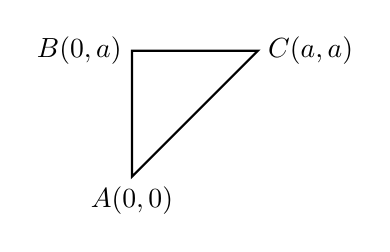
\begin{tikzpicture}[scale=0.8, thick]
    \coordinate (A) at (0,0);
    \coordinate (B) at (0,2);
    \coordinate (C) at (2,2);
    \draw (A) -- (B) node[midway, left] {} -- (C) node[midway, above] {} -- cycle;
    \node[below] at (A) {$A(0,0)$};
    \node[left] at (B) {$B(0,a)$};
    \node[right] at (C) {$C(a,a)$};
\end{tikzpicture}
\end{center}

\noindent then
\[
\int_{\vec{AC}} d\phi = \int_{[0,a]} d\theta = \int_0^a \theta'(s)\,ds = \theta(a) - \theta(0) := 2\pi i_\alpha
\]
Since by Green's Theorem,
\[
\oint_{\partial\Delta} d\phi = \oint_{\partial\Delta} \frac{\partial \phi}{\partial u}\,du + \frac{\partial \phi}{\partial v}\,dv \xlongequal{\text{Green's}} \iint_{\Delta} \left( \frac{\partial^2 \phi}{\partial v \partial u} - \frac{\partial^2 \phi}{\partial u \partial v} \right) du\,dv = 0
\]
then for computing $i_\alpha$, we can compute $\int_{\vec{AB}} d\phi$ and $\int_{\vec{BC}} d\phi$ separately.

\noindent On $\vec{AB}$, since by the above remark, we WLOG let

\begin{center}
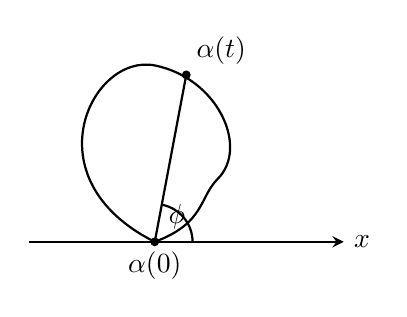
\begin{tikzpicture}[scale=0.8, >=stealth, thick]
    % Axes
    \draw[->] (-2,0) -- (3,0) node[right] {$x$};
    
    % Closed curve lying on x-axis
    \draw[thick] (0,0) .. controls (-2,1) and (-1,3) .. (0,2.8)
                       .. controls (1,2.6) and (1.5,1.5) .. (1,1)
                       .. controls (0.7,0.7) and (0.8,0.3) .. (0,0);
    
    % Points
    \fill (0,0) circle (2pt) node[below] {$\alpha(0)$};
    \fill (0.5,2.65) circle (2pt) node[above right] {$\alpha(t)$};
    
    % Secant Line
    \draw[thick] (0,0) -- (0.5,2.65);
    
    % Angle phi
    \draw (0.6,0) arc (0:79:0.6);
    \node at (0.35,0.4) {$\phi$};
\end{tikzpicture}
\end{center}

\noindent then
\[
\int_{\vec{AB}} d\phi = \begin{cases}
\pi - 0, & \text{counterclockwise} \\[5pt]
0 - \pi, & \text{clockwise}
\end{cases}
\]

\noindent Similarly, on $\vec{BC}$,

\begin{center}
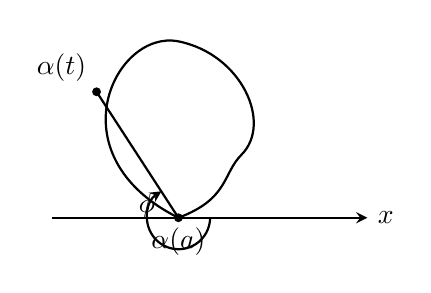
\begin{tikzpicture}[scale=0.8, >=stealth, thick]
    % Axes
    \draw[->] (-2,0) -- (3,0) node[right] {$x$};
    
    % Closed curve lying on x-axis touching at alpha(a)
    \draw[thick] (0,0) .. controls (-2,1) and (-1,3) .. (0,2.8)
                       .. controls (1,2.6) and (1.5,1.5) .. (1,1)
                       .. controls (0.7,0.7) and (0.8,0.3) .. (0,0);
    
    % Points
    \fill (0,0) circle (2pt) node[below] {$\alpha(a)$};
    \fill (-1.3,2.0) circle (2pt) node[above left] {$\alpha(t)$};
    
    % Secant Line
    \draw[thick] (0,0) -- (-1.3,2.0);
    
    % Angle phi (Explementary Angle: from positive x-axis counterclockwise to secant line)
    \draw[<-] (-0.27, 0.42) arc (123:360:0.5);
    \node at (-0.5, 0.2) {$\phi$};
\end{tikzpicture}
\end{center}

\noindent we have
\[
\int_{\vec{BC}} d\phi = \begin{cases}
2\pi - \pi, & \text{counterclockwise} \\[5pt]
\pi - 2\pi, & \text{clockwise}
\end{cases}
\]

\noindent Hence, $i_\alpha = 1$, counterclockwise \quad or \quad $i_\alpha = -1$, clockwise. 
\end{proof}

\begin{corollary}
\[
\int_\alpha K(s)\,ds = 2\pi \quad \text{or} \quad -2\pi
\]
\end{corollary}

\begin{proof}
It's immediately from the Hopf's Theorem and the computation
\[
i_\alpha := \frac{1}{2\pi}(\theta(a) - \theta(0)) = \frac{1}{2\pi}\int_0^a \theta'(s)\,ds = \frac{1}{2\pi}\int_0^a K(s)\,ds = \frac{1}{2\pi}\int_\alpha K(s)\,ds. \qedhere
\]
\end{proof}

\noindent\textbf{Remark:} \begin{itemize}
    \item In fact, for any closed spatial curve $\alpha$, the total curvature satisfies that
\[
\int_\alpha K(s)ds \geq 2\pi \text{ or } \leq -2\pi
\]
where the equality holds iff $\alpha$ is a plane curve.

    \item If a simple closed curve $\alpha$ has strictly positive curvature, then $\alpha$ is strictly convex.
\end{itemize}

\subsection{Isoperimetric Inequality}

\lemma{Area Formula}\\
Let $\alpha$ be a simple, closed plane curve bounding a region $R$. Anti-clockwise, the area $A$ of $R$ is equal to
\[
A = \int_\alpha x\,dy = -\int_\alpha y\,dx
\]

\begin{proof}
The second equality is directly by Green's Thm. \quad$\square$
\end{proof}

\theorem{Isoperimetric Inequality}\\
Let $\alpha$ be a simple, closed plane curve of length $\ell$ and let $A$ be the area bounded by $\alpha$. Then
\[
\ell^2 \geq 4\pi A
\]
where the equality holds iff $\alpha$ is a circle.

\begin{proof}
WLOG, let $\alpha(s) = (x(s), y(s))$ be a p.a.l., so $\alpha(\ell) = \alpha(0)$. Let $E$ and $E'$ be two parallel lines which do not meet $\alpha$ and lie on either side of $\alpha$. Then move them together until they first meet $\alpha$. We hence obtain two parallel tangent lines $L$ and $L'$ to $\alpha$, so that $\alpha$ is entirely between $L$ and $L'$. Consider a circle which is tangent to both $L$ and $L'$ and does not meet $\alpha$. Then take a coordinate system with origin at the center of the circle and $x$-axis perpendicular to $L$ and $L'$.

\begin{center}
\begin{tikzpicture}[scale=0.8]
% parallel lines
\draw (2,0) -- (2,6);   % E
\draw (4.5,0) -- (4.5,6); % L
\draw (6.5,0) -- (6.5,6); % L'
\draw (9,0) -- (9,6);   % E'
% labels with arrows
\node at (1.5,6.2) {$E$};
\draw[->] (2.2,5.8) -- (2.7,5.8);
\node at (4.7,6.2) {$L$};
\node at (6.9,6.2) {$L'$};
\node at (9.5,6.2) {$E'$};
\draw[->] (9.3,5.8) -- (8.8,5.8); % arrow pointing LEFT
% curve alpha tangent to L at (4.5,4.8) and to L' at (6.5,4.8)
\draw (4.5,4.8) .. controls (4.9,5.6) and (6.1,5.6) .. (6.5,4.8)
.. controls (6.1,4.0) and (4.9,4.0) .. (4.5,4.8);
\node at (5.5,4.8) {$A$};
\node at (5.0,5.5) {$\alpha$};
% circle tangent to both L and L' (radius = half the distance between them)
\draw (5.5,1.2) circle (1);
\fill (4.5,1.2) circle (1.2pt); % tangency point on L
\fill (6.5,1.2) circle (1.2pt); % tangency point on L'
% axes: origin at center of circle, x-axis perpendicular to L and L'
\draw[->] (5.5,1.2) -- (5.5,3) node[above] {$y$};
\draw[->] (5.5,1.2) -- (7.3,1.2) node[right] {$x$};
\end{tikzpicture}
\end{center}

\noindent Denote $\alpha\cap L =: \{\alpha(s_0)\}$ for some $0 < s_0 < \ell$ and $\alpha\cap L' =: \{\alpha(0)\}$ (assuming). Then parametrize the circle by $\beta(s) = (z(s), w(s))$, $0\le s\le \ell$, where
\[
z(s) := x(s) \quad\text{and}\quad w(s) := \begin{cases}\sqrt{r^2 - x^2(s)}\,, & \text{if } 0\le s\le s_0\\ -\sqrt{r^2 - x^2(s)}\,, & \text{if } s_0\le s\le \ell\end{cases}
\]
(where $r$ denotes the radius of the circle). Then by lemma above, we have:
\[
A = \int_\alpha x\,dy = \int_0^\ell x(s)\cdot\frac{dy}{ds}(s)\,ds = \int_0^\ell xy'\,ds
\]
and
\[
\pi r^2 = -\int_\beta w\,dz = -\int_0^\ell wz'\,ds
\]
Hence, compute:
\[
A + \pi r^2 = \int_0^\ell (xy' - wz')\,ds = \int_0^\ell (xy' - wx')\,ds = \int_0^\ell \langle (x', y'), (-w, x)\rangle\,ds
\]
\[
\stackrel{(*)}{\leq} \int_0^\ell \left|\langle (x', y'), (w, x)\rangle\right| ds \stackrel{(**)}{\leq} \int_0^\ell |(x', y')|\cdot|(-w, x)|\,ds
\]
where $(**)$ holds by the Cauchy-Schwarz inequality. Since $\alpha$ is p.a.l., then $|(x', y')| = 1$. Since $z(s) = x(s)$ and $(z, w)\in$ circle of radius $r$, then $|(-w, x)| = r$. Thus, $A + \pi r^2 = \int_0^\ell 1\cdot r\,ds = r\cdot\ell$. Therefore,
\[
r\cdot\ell \geq A + \pi r^2 \stackrel{(***)}{\geq} 2\sqrt{A\pi r^2} \Rightarrow \ell^2 \geq 4\pi A.
\]
For the condition of equality, it suffices to show that the inequalities $(*)$, $(**)$, and $(***)$ all hold exactly when $\alpha$ is a circle.

\noindent ($\Leftarrow$): We suppose first that $\alpha$ is a circle. Then $A = \pi r^2$, $\ell = 2\pi r$, so we're done.

\noindent ($\Rightarrow$): Suppose that $(*)$, $(**)$, and $(***)$ are all equalities. Then
\[
(*)\ \checkmark \Rightarrow \langle (x', y'), (-w, x)\rangle \geq 0
\]
\[
(**)\ \checkmark \Rightarrow (x', y') = \lambda(-w, x)\ \text{with}\ |\lambda| = \frac{1}{r}
\]
\[
\Rightarrow \lambda = \frac{1}{r} \stackrel{\substack{\text{ODE}\\ x^2+w^2=r^2}}{\Longrightarrow} x^2 + (y - c)^2 = r^2\quad\text{for some constant } c. 
\]
\end{proof}
